\section{Разработка программного средства}
\label{sec:development:intro}

При построении данного дипломного проекта необходимо использовать некоторые основные компоненты от Spring Cloud и Netflix ОSS, позволяющие отдельно разворачивать микросервисы, а также наладить общение между ними без ручного управления. 

В итоге для создания нового экземпляра микросервиса и сбалансирования нагрузки нужно будет выполнить только несколько команд, чтобы начать использовать его без каких-либо ручных настроек.


\subsection{Язык программирования Java}
\label{sub:development:java}
В качестве основного языка программирования была выбрана Java, так как это статически компилируемый язык программирования, проверенные временем и имеющий огромное количество написанных под него библиотек и фреймворков. 

JVM оптимизирована для больших многоядерных машин, и она без проблем может управлять сотнями потоков, благодаря чему позволяет строить высокопроизводительные системы.

Существование JVM-подобных языков, таких как Groovy, Scala, Clojure является так же большим плюсом. Благодаря им, и тому что они полностью JVM совместимы, при разработки на java необязательно использовать только её, зачастую удобно совмещать несколько JVM-подобных языков программирования, чтобы в тех или иных случаях, получать преимущества получать преимущества того или иного языка.   

Благодаря фрэймворку Spring, и в частности его проекта Spring Cloud, java удобно использовать в построении микросервисной архитектуры, что является большим плюсом для данного программного средства, так как оно построено на ней. 

Также стоит отметить, что язык Java имеет превосходную среду разработки IntelliJ Idea, которая позволяет удобно и быстро разрабатывать программные средства.


\subsection{Spring Cloud и Netflix OSS}
\label{sub:development:netflix}

Spring Cloud ~\cite{spring_cloud} это достаточно новый продукт из экосистемы spring.io ~\cite{spring_site} с набором компонент которые удобно использовать для построения микросервисной архитектуры. В значительной степени Spring Cloud базируется на компонентах от Netflix OSS ~\cite{netflix_oss}.

Spring Cloud интегрирует компоненты Netflix в экосистему Spring используя автоматическую конфигурацию и конвенцию вместо обычной конфигурации подобно тому, как работает Spring Boot.

Приведенный ниже рисунок~\ref{fig:common-comp} отображает общие компоненты для реализации отдельных микросервисов ~\cite{tut_micros}:

\begin{figure}[ht]
\centering
  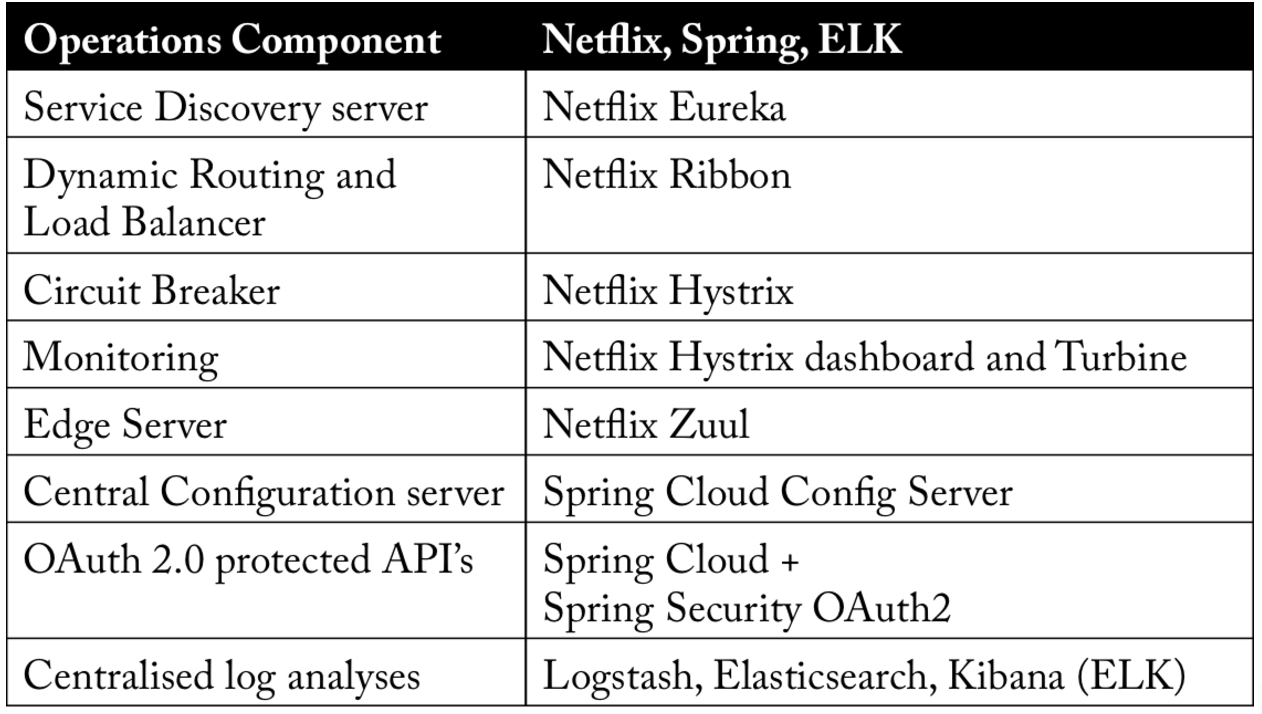
\includegraphics[scale=0.6]{common-comp.png}  
  \caption{Общие компоненты для реализации отдельных микросервисов}
	\label{fig:common-comp}
\end{figure} 



Netflix Eureka -- Service Discovery Server позволяет микросервисам регистрировать себя во время выполнения, так они появляются в микросервисной архитектуре ~\cite{eureka}.

Netflix Ribbon -- динамическая маршрутизация и балансировки нагрузки может быть использована для поиска экземпляра микросервиса для выполнения операции во время выполнения. Netflix Ribbon использует информацию, доступную в Eureka, чтобы найти соответствующие экземпляры служб. Если более чем один экземпляр найден, Netflix Ribbon будет применяться для балансировки нагрузки, чтобы распределить запросы по имеющимся экземплярам. Netflix Ribbon не является отдельным сервисом, но вместо этого используется в качестве встроенного компонента в других микросервисах ~\cite{ribbon}.

Netflix Zuul -- Edge Server Zuul это gateway с внешним миром, он не допускает каким-либо несанкционированным внешним запросам пройти в систему.  Edge Server также обеспечивает хорошо известную точку входа к какому-либо микросервису в микросервисной архитектуре. Использование динамически выделенных портов удобно для избежания конфликтов портов и для того чтобы свести к минимуму администрирование. Zuul использует Ribbon для поиска доступных микросервисов и маршрутов и отправляет внешний запрос к соответствующему экземпляру службы ~\cite{zuul}. 

Netflix Hystrix -- Circuit breaker Netflix Hystrix предоставляет возможности автоматического перенаправления вызова если произошли какие-либо проблемы с тем или иным микросервисом. Если микросервис не отвечает (например, из-за тайм-аута или ошибки связи), Hystrix может перенаправить вызов на внутренний метод запасного варианта. Если служба неоднократно не в состоянии ответить, Hystrix будет размыкать цепь вызывая внутренний аварийный метод, не пытаясь вызвать службу на каждом последующем вызове, пока сервис снова не станет доступным. Для того, чтобы определить, является ли сервис снова доступным Hystrix позволяют некоторым запросам попробовать достучатся до сервиса, даже если цепь была разорвана. Hystrix вводится как встроенный компонент в каждый отдельный микросервис ~\cite{hystrix}.

Netflix Hystrix dashboard and Netflix Turbine - специальное средство для мониторига статусов сервисов Hystrix. Оно обеспечивает графическое представление информации о состояниях всех сервисов, на основе информации, содержащейся в Eureka ~\cite{hystrix}. 

При реализации данного программного средства были построены следующие микросервисы:

Ets-service -- основной сервис в котором реализовано ядро с работой над событиями. Оно предоставляет API по созданию различных событий и их отслеживанию. 
Для хранения структуры различных событий используется реляционная база даны PostrgreSQL в которой описаны параметры событий, их типы, доступные значения, значения по умолчанию, наличие обязательности тех или иных полей и другая информации характеризующие то или иное событие.
Для отслеживания же самих событий используется NoSql база данных Mongo ~\cite{mongo}. Она лучше всего подходит для этой цели потому что, является быстрой бесструктурной документно-ориентированной базой данных, что позволят сохранять любые события созданные пользователем, а также изменять их в любое время
Отслеживание события происходит через предоставленное API. Перед тем как оно будет записано, происходит проверка на то что событие корректно, что осуществляется с помощью проверки его структуры. Для проверки же структуры все события подгружаются в Redis (высокопроизводительное не реляционное распределённое хранилище данных).


Administration-client -- сервис разработанный для администраторов и менеджеров в нем можно настраивать/редактировать/добавлять новые события, следить за их статистикой как за определенный период так и в режиме онлайн. 
Пользовательский интефейс разработан отдельно на Angular. 
Также стоит отметить что все API документируется с помощью Swagger, что позволяет frontend разработчикам сгенерировать нужное им API для обращения к построенной системе.


Salesforce-integration -- сервис, предоставляющий интеграцию с СRM системой Salesforce. В  котором также разработана интеграция  онлайн чата с клиентом, с сохранением соответствующие  события с помощью Ets-service.


Social-integration -- микросервис, разработанный для собирания публичной информации о пользователе, включающий в себя интеграцию с внешним сервисом публичной информации FullContact, который помогает в сборе информации из доступных социальных сетей, фотографий, географического положения, карьере и около 100 других различных данных о пользователе.


Discovery-server -- этот сервис позволяет микросервисам обнаруживать друг друга и общаться между собой (в данном случае использовалась Eureka).


Config-server -- это сервис, использующий Spring Cloud Config для централизованного хранения конфигурации всех микросервисов в отдельном git репозитории.

Во всех микросевисах использовался Hystrix для случаев, когда какой-то из них откажет. Данный же сервис предоставляет возможность графического мониторинга состояния всех микросервисов.


На рисунке~\ref{fig:save-event} изображен Hystrix Dashboard разрабатываемого программного средства.
\begin{figure}[ht]
\centering
  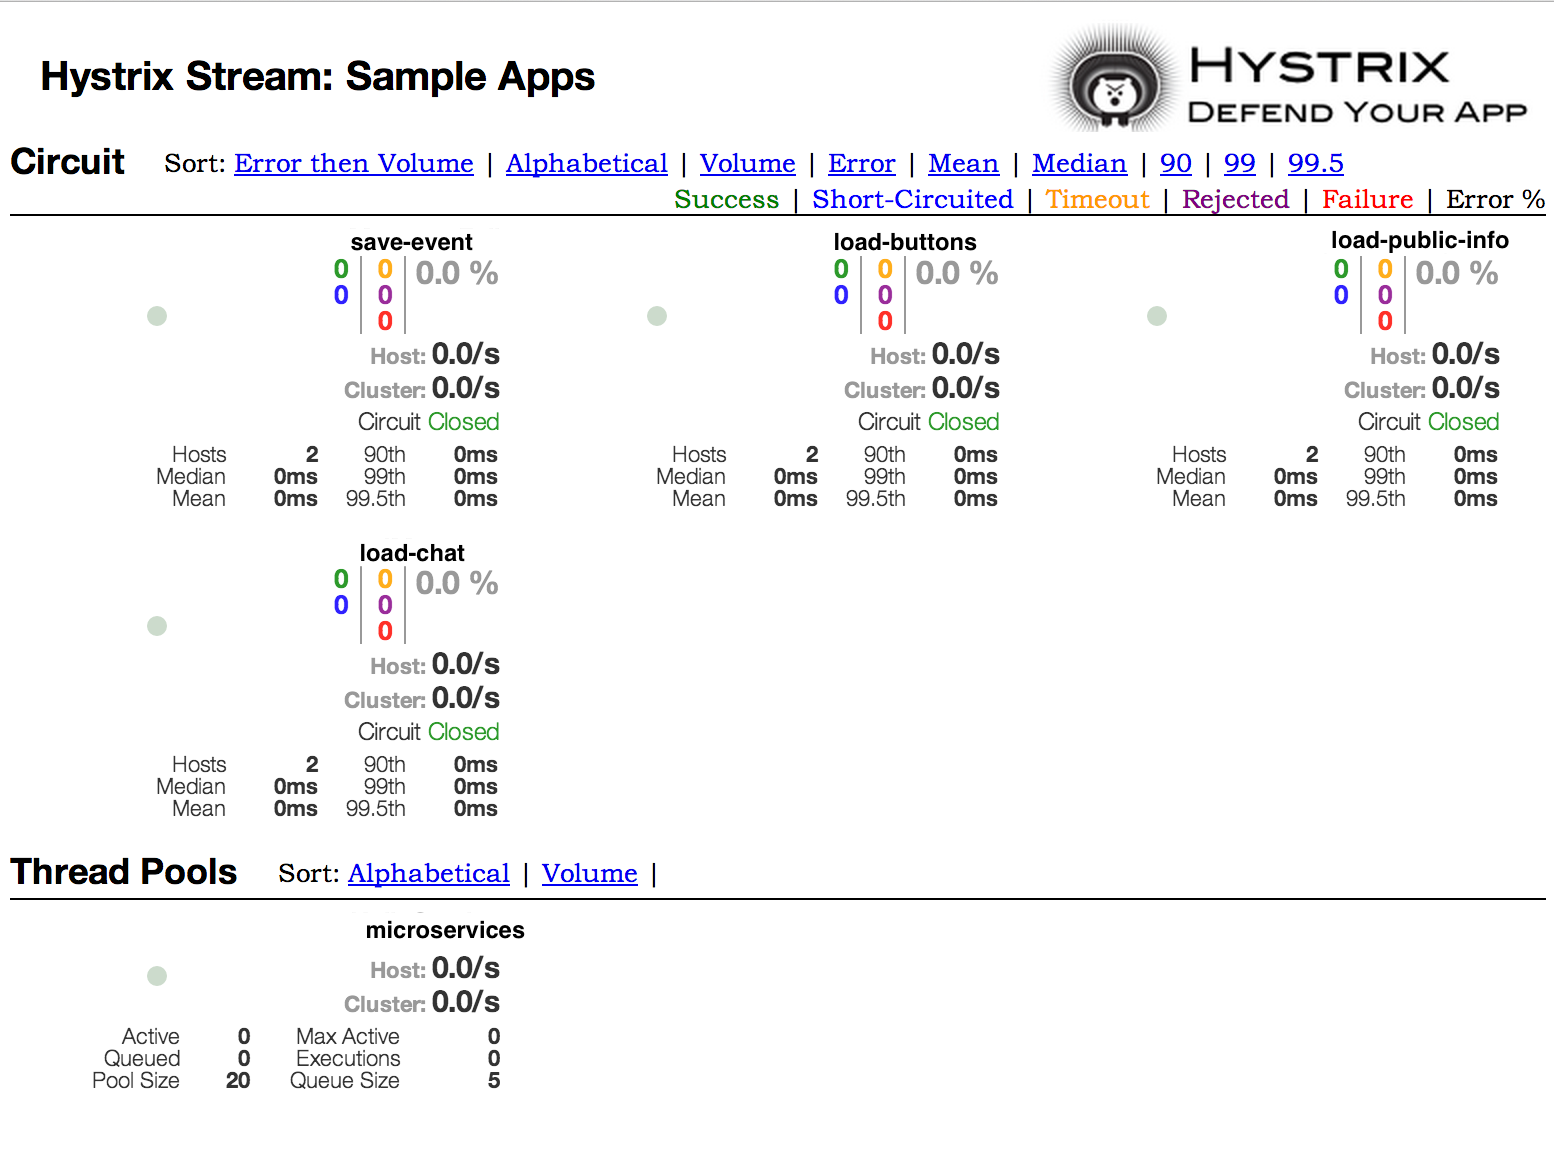
\includegraphics[scale=0.2]{hystrix.png}  
  \caption{Hystrix Dashboard программного средства}
  \label{fig:hystrix}
\end{figure} 



Gateway -- микросервис, использующий Netflix Zuul для предоставления централизованной точки доступа к микросервисам, также с помощью него и Spring Cloud Security настроена безопасность для всех микросервисов.


Для развертывания микросервисов используется docker и docker-compose.
С помощью них можно горизонтально масштабировать любой микросервис одной командой. 

Например одной командой docker-compose scale ets-service=5, поднимется 5 экземпляров микросервиса ets-service, и с помощью Ribbon другие микросервисы будут балансировать нагрузку по ним при обращении к сервису ets-service.


\subsection{Алгоритм сохранения события}
\label{sub:development:save_event}
Запросы на сохранение события, как и все остальные, сначала посылаются в микросервис gateway. В нем выполняется базовая аутентификация, которая проверяет, чтобы запросы обрабатывались только от клиентов, обладающих на это правами. Далее запрос отправляется с помощью Zuul Proxy в ets microservice, в котором находится логика обработки событий.

В самом же ets микросервисе событие о сохранении сразу же помещается в очередь сообщений RabbitMQ, таким образом все последующие действия выполняются асинхронно, и на стороне пользователя нету задержки, связанной с сохранением событий. Тем временем обработчик очереди событий RabbitMQ, постепенно обрабатывает все прилетевшие в него сообщения. Он же, в свою очередь, сначала пытается распознать к какому из типов моделей событие относится, то или иное сообщений, после чего, если тип найден, сохраняет событие его в MongoDB (рисунок~\ref{fig:save-event}).

После этого посылается ещё одно сообщение в RabbitMQ, теперь уже о результатах сохранения события, благодаря чему, все последующие действия опять выполняются асинхронно .
Обработчик сообщений предназначенный для обработки результатов сохранения в RabbitMQ, в свою очередь сохраняет результаты статистики и агрегирует их за последнее время по заданным критериям в системе. После чего эти данные отправляются в панель администратора, через вебсокеты, для того чтобы в ней можно было следить за происходящими событиями на сайте в режиме реального времени .%(рисунок~\ref{fig:save-event}). 

% На рисунке~\ref{fig:save-event} изображен алгоритм сохранения события.

\pagebreak
\begin{figure}[h]
\centering
  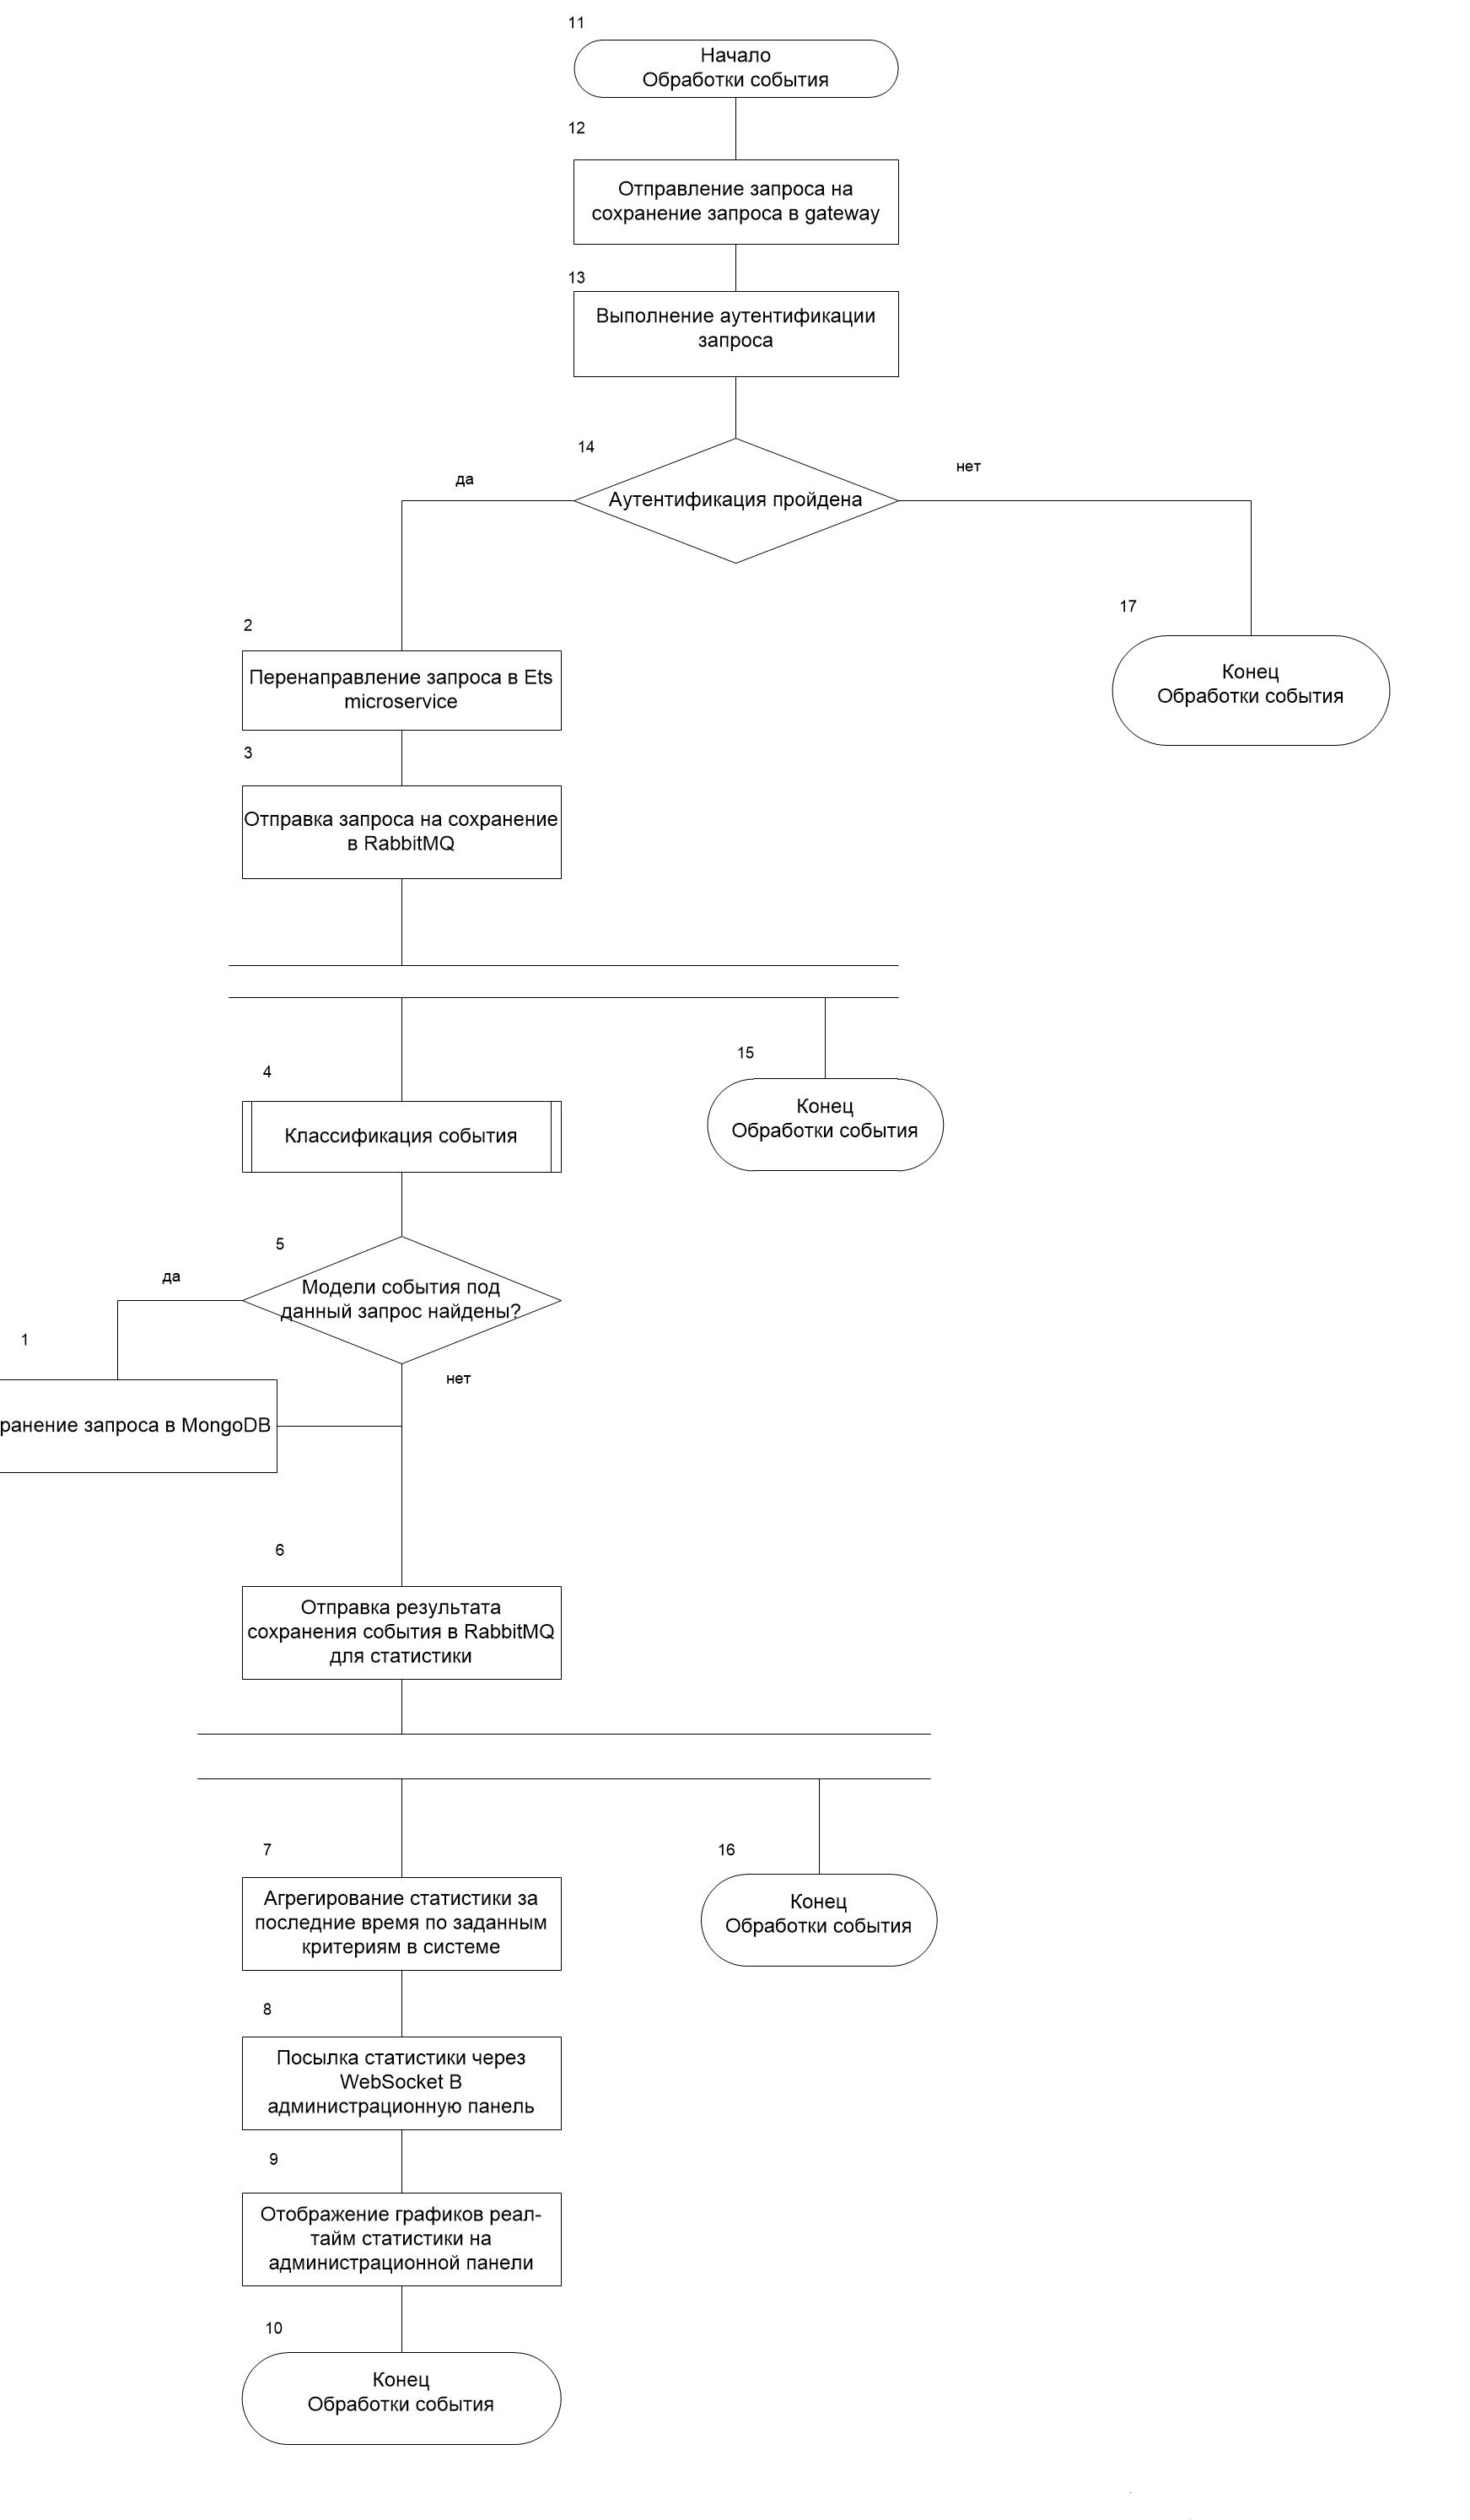
\includegraphics[scale=0.22]{save-event.png}  
  \caption{Алгоритм сохранения события}
  \label{fig:save-event}
\end{figure} 

\subsection{Алгоритм классификации событий}
\label{sub:development:klassific}
Все модели событий, которые принимает наша система, должны быть описаны в реляционной базе данных (в нашем случаем PostgreSQL) и их можно добавлять, удалять и изменять в любое время. 

Описание каждой модели включает в себя тип и набор полей, которые в неё входят. А каждое поле, в свою очередь, содержит информацию, к какому типу оно должно принадлежать(Date, Double, String, Long, List) и то, обязательно оно или нет (рисунок~\ref{fig:ets-domain}). 

% На рисунке~\ref{fig:ets-domain} приведена схема диаграмма классов модели событий.

\begin{figure}[h]
\centering
  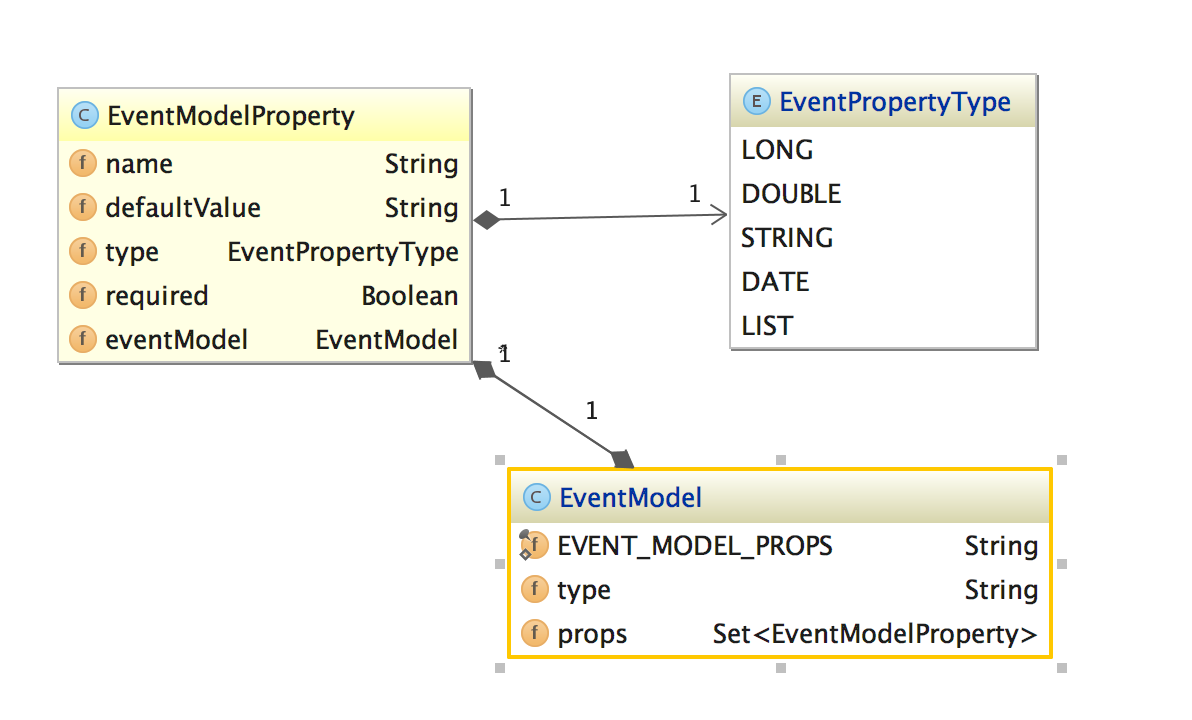
\includegraphics[scale=0.6]{ets-domain.png}  
  \caption{Диаграмма классов модели событий}
  \label{fig:ets-domain}
\end{figure} 


Алгоритм классификации событий определяет, к каким моделям событий можно соотнести пришедшее на вход событие, чтобы тип совпадал и все валидации проходили.
Первое что нужно алгоритму, это все модели данных, но так как все время обращаться в реляционную базу за ними было бы очень дорого и неэффективно, все модели подгружаются в in memory базу Redis ~\cite{redis}. Для того, чтобы данные в ней были все время актуальны, на ней настроен TTL, и поэтому через n-ое время все модели событий обновляются и всё время являются актуальными.

Сначала алгоритм ищет все модели событий у которых тип соответствует полю типа входного события, далее он идет по всем полям модели события, и проверяет, что пришедшее событие подходит под его модель: проверяет все обязательные поля и типы полей. Таким образом данный алгоритм находит все модели которые подходят для пришедшего события, а также валидирует их (рисунок~\ref{fig:klassification-event}).

% На рисунке~\ref{fig:klassification-event} приведена схема алгоритма классификации события.

\pagebreak
\begin{figure}[h]
\centering
  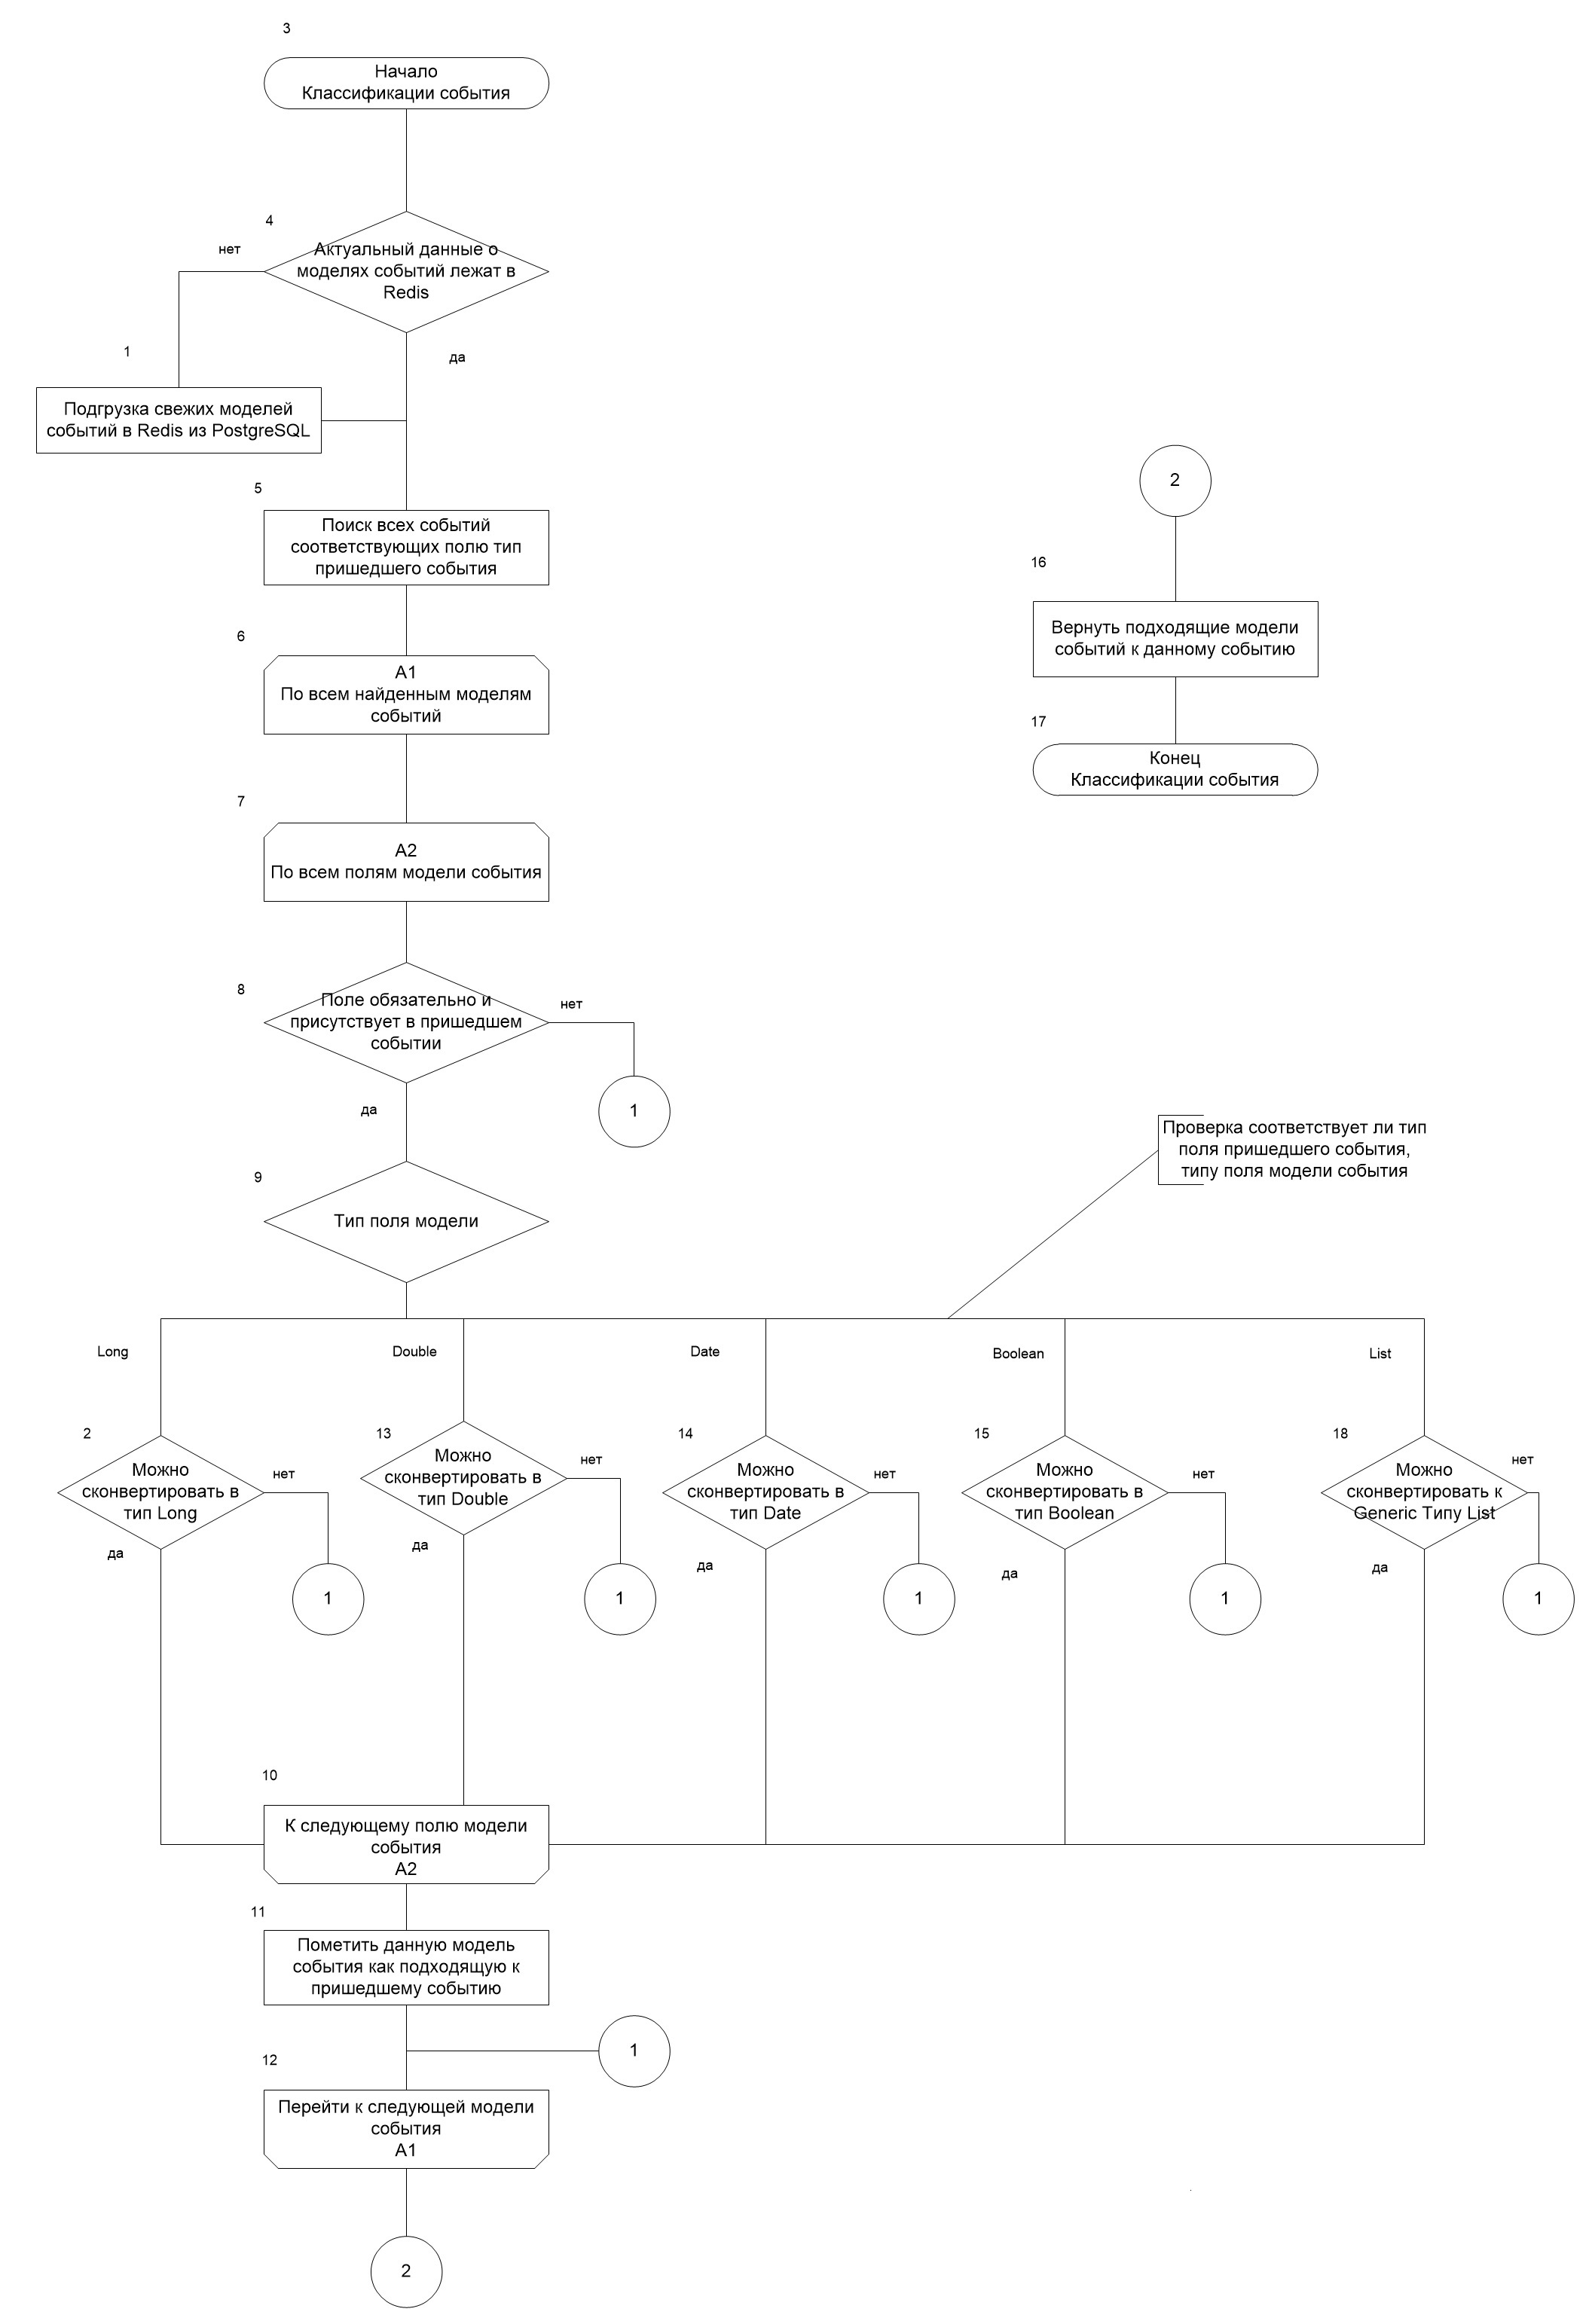
\includegraphics[scale=0.22]{klassification-event.jpg}  
  \caption{Алгоритм классификации события}
  \label{fig:klassification-event}
\end{figure} 



\subsection{Схема интеграции с онлайн чатом Salesforce}
\label{sub:development:chat}
Рассмотрим схему алгоритма интеграции с онлайн-чатом Salesforce ~\cite{live_agent}. 

Для интеграции c онлайн чатом Salesforce нужны стандартные объекты Salesforce, такие как LiveChatButton, DeploymentID и OrganizationID. Они включают в себя большое количество опций прямо из коробки Salesforce. Их описание можно найти в соответсвующей документации по SF. Отметим только, что LiveChatButton связывается с DeploymentID, и SF при подгрузке пытается подгрузить все LiveChatButton по соответствующим условиям, описанным в SF. Также на LiveChatButton есть связь со SkillID, по которому тоже можно фильтровать то, какие из кнопок должны подгружаться.

Дополнительно в SF были созданы собственные объекты Site и Relative URL. В первом размещается общая информация о сайте и главное его домен и сниппет. Во втором есть связь с сайтом, DeploymentID, SkillID, Callback и относительная страница, но которую эти настройки должны применятся. После того, как SF сконфигурирован, в него могут заходить агенты и приступать к своей работе (общению с пользователями сайта, собиранию статистик, настройке новых страниц, в Salesforce CRM можно делать очень многое). 

На рисунке~\ref{fig:sf-domain} приведена схема диаграмма классов интеграции с Salesforce.

\begin{figure}[h]
\centering
  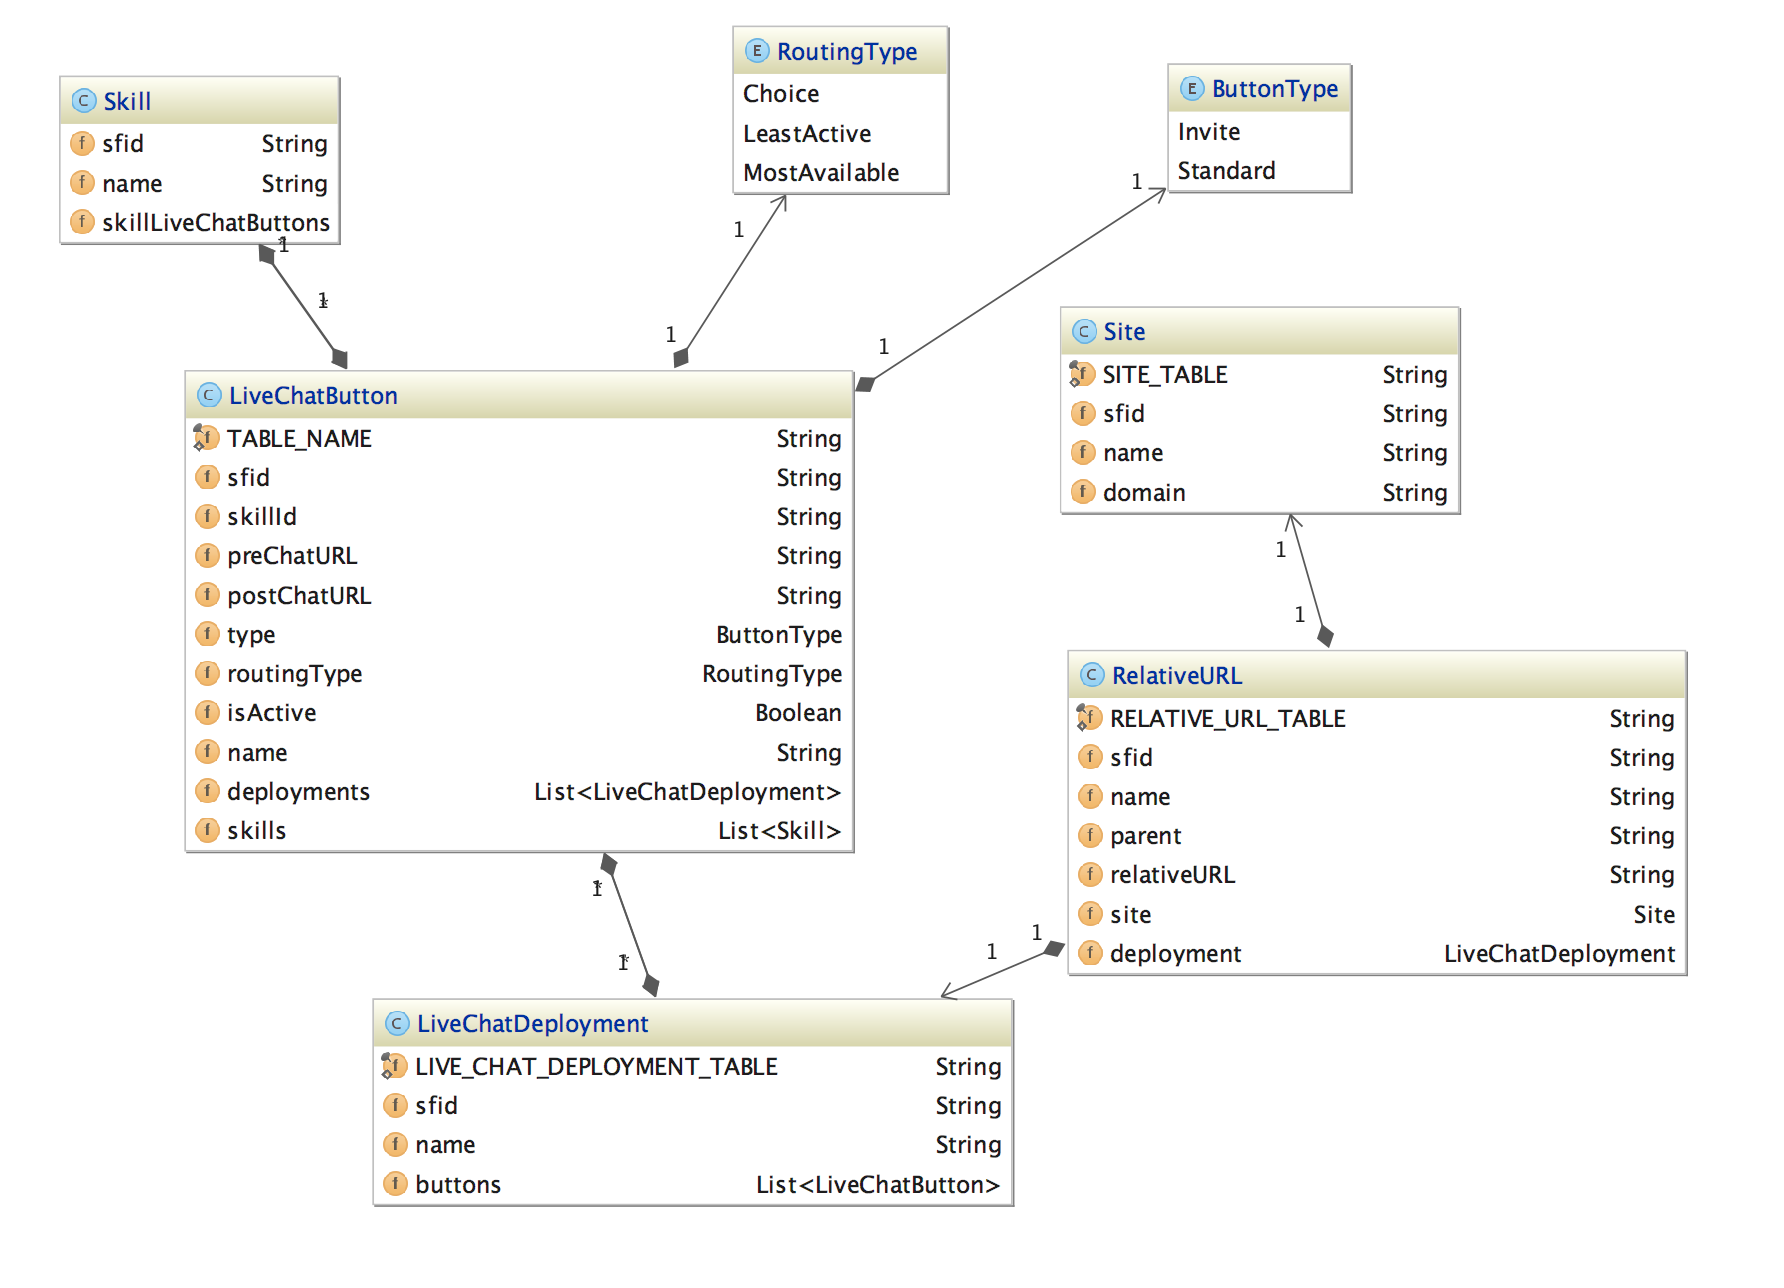
\includegraphics[scale=0.4]{sf-domain.png}  
  \caption{Диаграмма классов интеграции с Salesforce}
  \label{fig:sf-domain}
\end{figure} 

Для интеграции с  сервисом, клиент должен разместить сниппет, который он может найти в Salesforce CRM. После того как сниппет подгрузится на странице пользователя, он делает запрос на извлечение данных необходимых для подгрузки онлайн чата. После того как сниппет был отправлен и аутентифицирован, запрос перенаправляется в salesforce-integration microservice. 

В нем определяется, с какой страницы был произведен запрос, и дальше ищется в базе синтегрированной с  SF, к какой связке (Site, RelativeURL) она больше всего подходит. Дальше из этой связки достаются нужные объекты OrganizationID, DeploymentId, SkillID и Callback. Следующий шаг -- это найти все подходящие LiveChatButton. Они определяются по найденным объектам DeploymentID и SkillID. После того, как вся нужная информация собрана (OrganizationID, DeploymentId, SkillID, Callback и список LiveChatButton) она передается в браузер клиенту, и в нём подгружается Salesforce онлайн-чат по пришедшим параметрам.

После того, как он подгрузился, выполняется дополнительный callback, переданный из SF, который позволяет выполнить любые дополнительные действия, нужные в тех или иных случаях. 

На рисунке~\ref{fig:chat-integration} приведена схема интеграции.
% \pagebreak
\begin{figure}[h]
\centering
  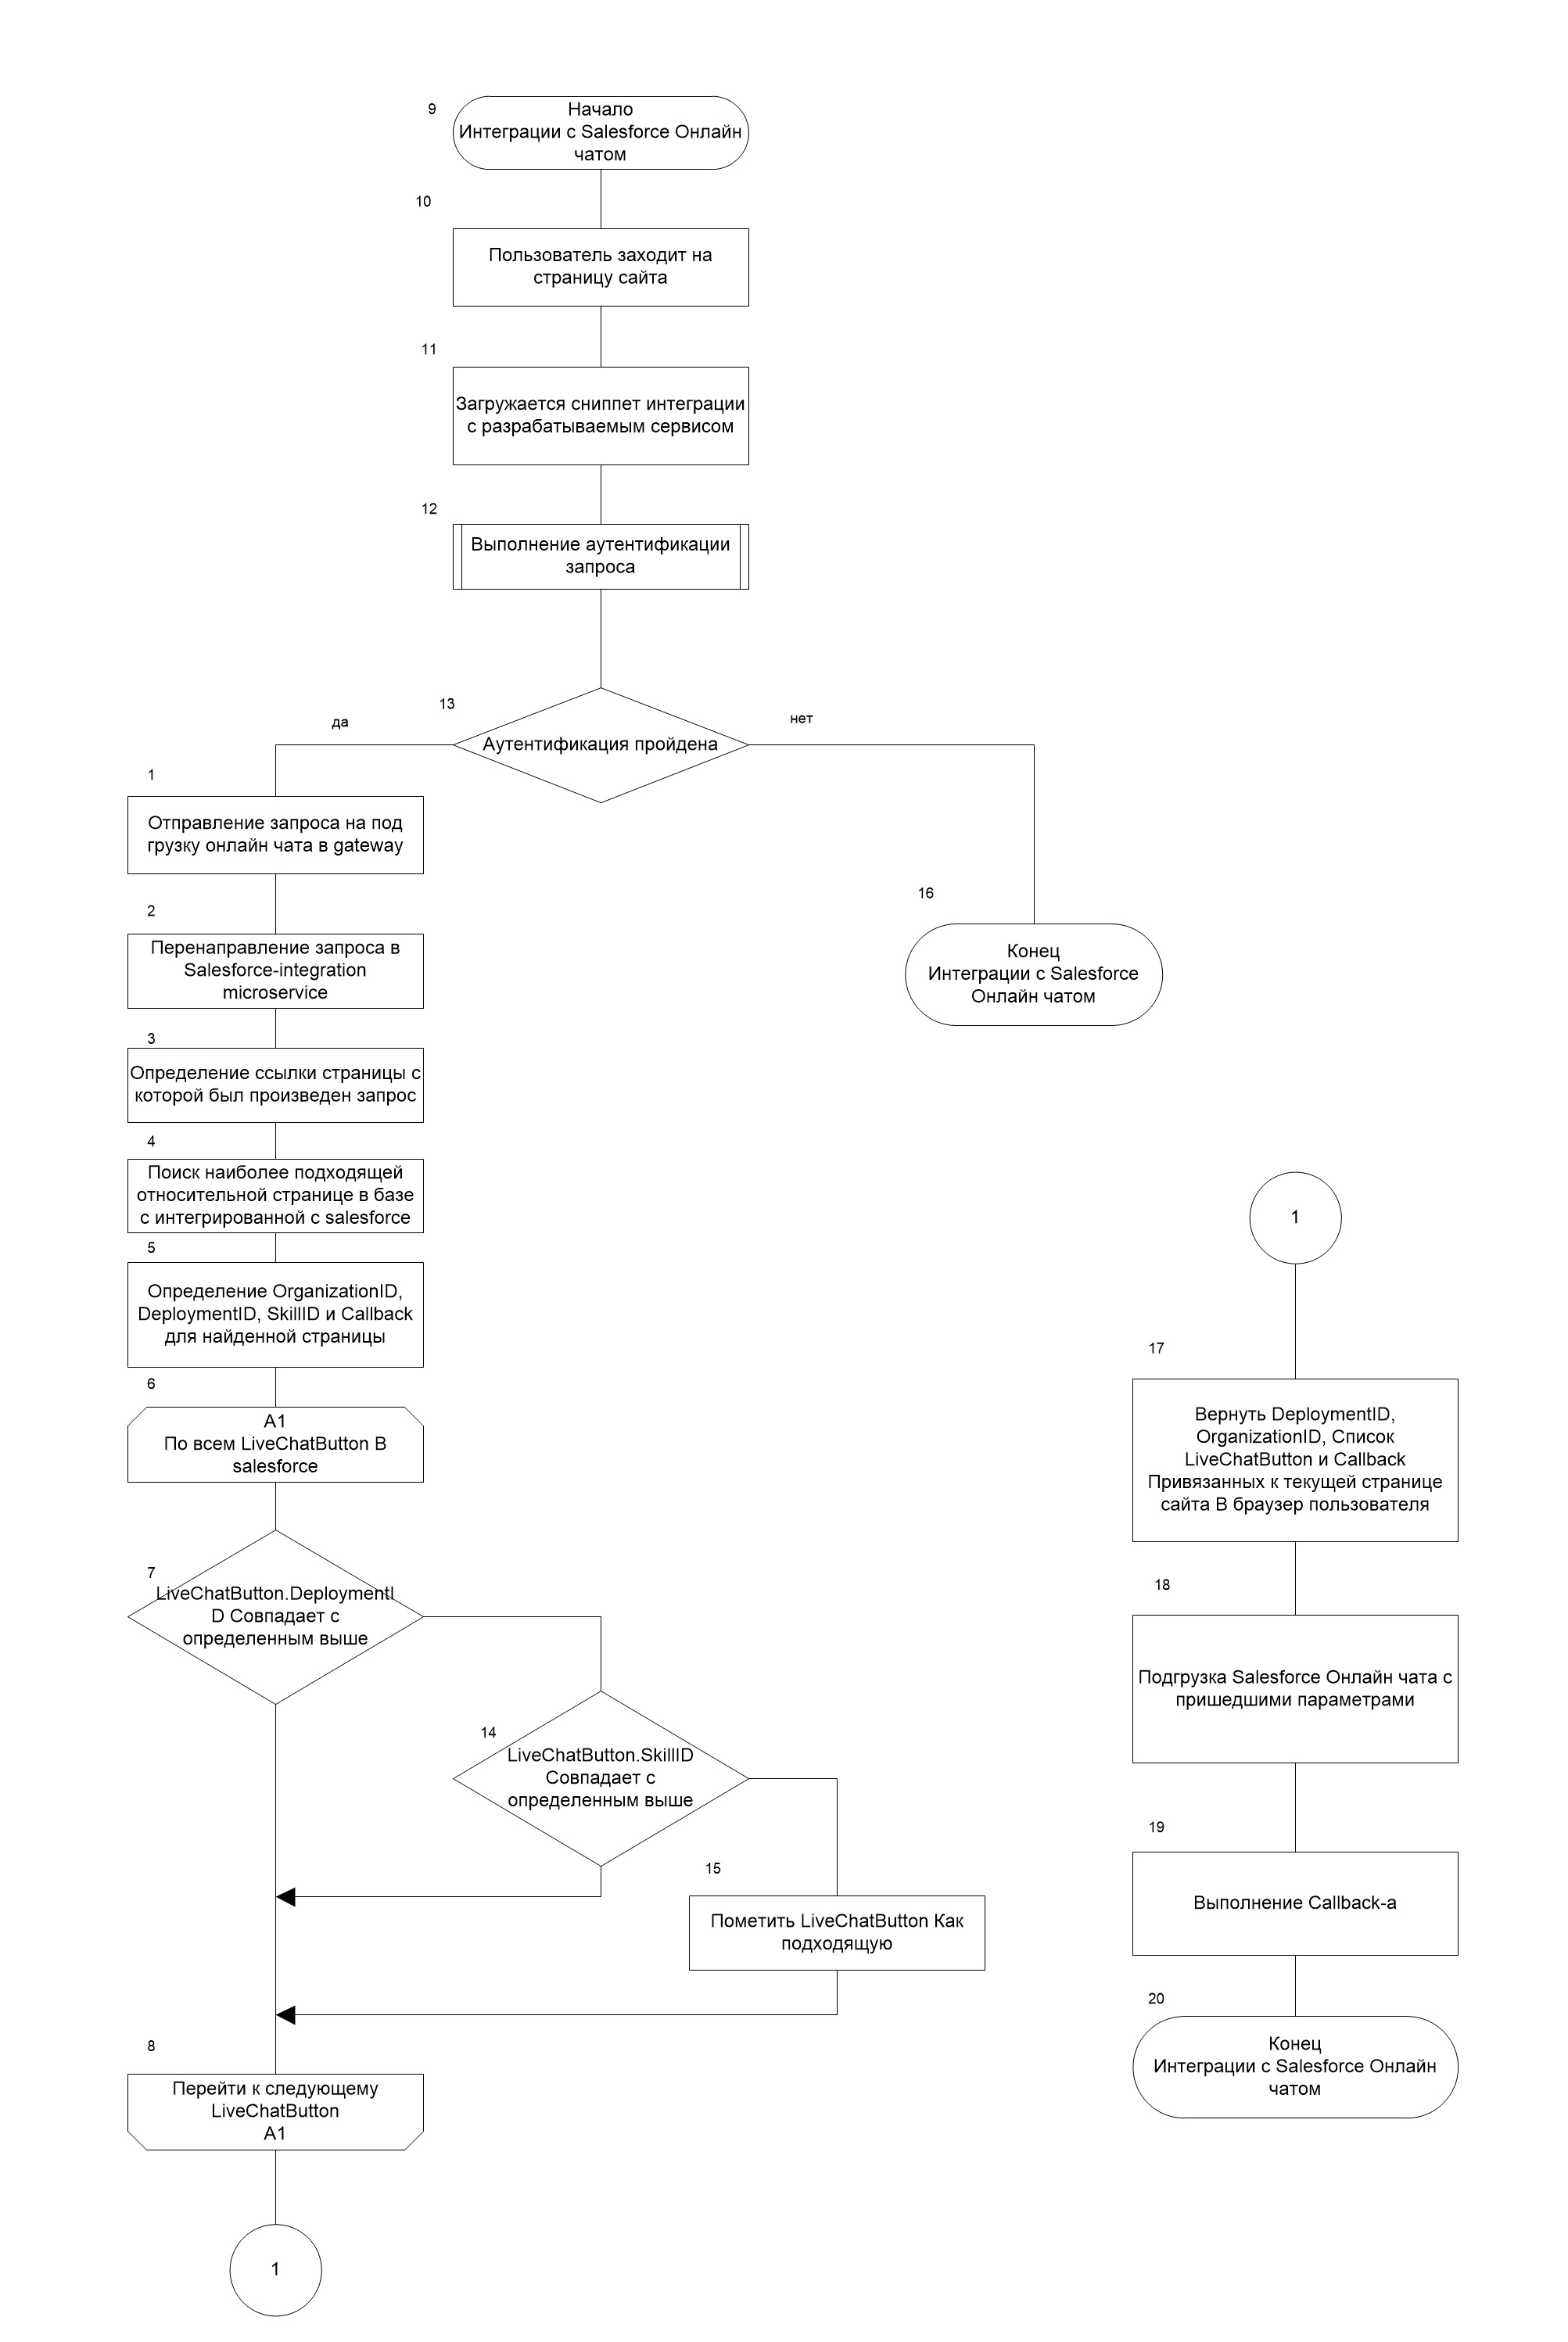
\includegraphics[scale=0.20]{sf-chat-integration.jpg}  
  \caption{Схема интеграции с Salesforce online chat}
  \label{fig:chat-integration}
\end{figure} 


